% ============================================================ NBMOs, disjointness
\section{NBMOs \& disjointness}

\begin{frame}{Borden \& Davidson's classification}
  \begin{columns}[c]
    \column{0.52\textwidth}
    \begin{paperclaim}
      ``If the two orbitals do not have common atoms and the probability of two electrons occupying the same space
      is nil independent of their spins, they are termed disjoint. Under such circumstances, the energy of an
      open-shell singlet can become comparable to or even lower than that of a triplet.'' (p.\ 443)
    \end{paperclaim}
    \onslide<2->{\small three things to derive: \cgold{(1)} how to find NBMOs, \cgold{(2)} when they can be disjoint,
      \cgold{(3)} why disjoint means $K\approx0$}
    \column{0.45\textwidth}
    \centering
    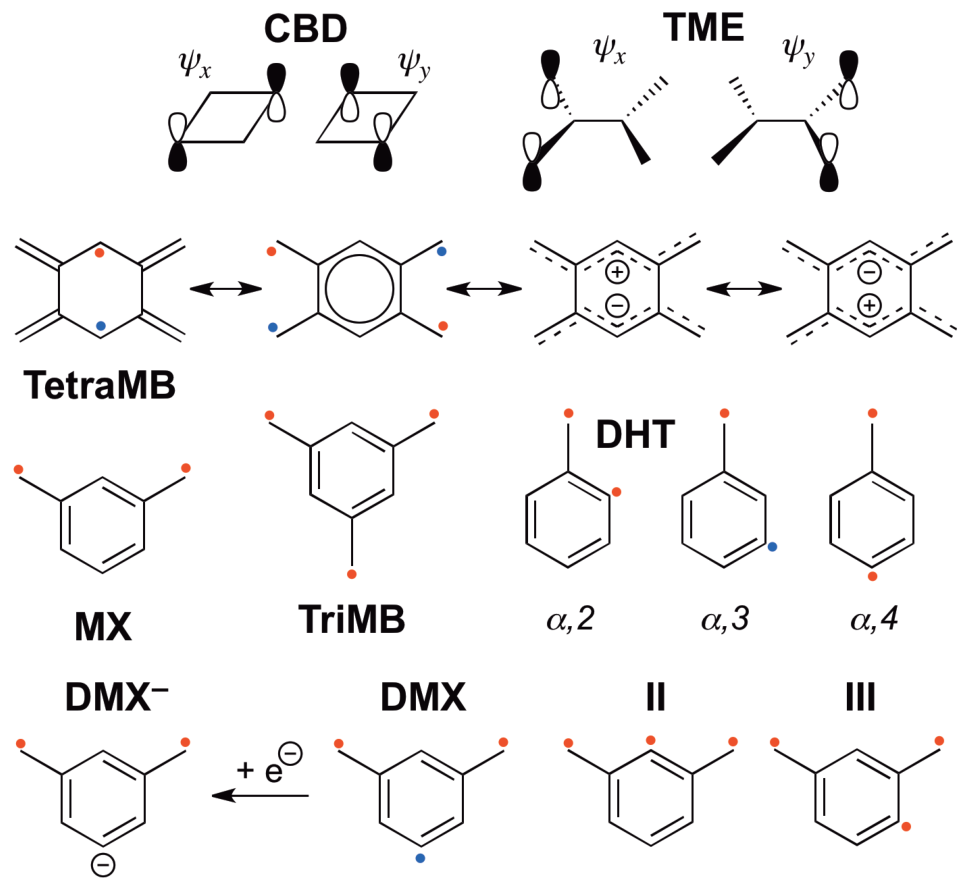
\includegraphics[width=0.95\linewidth]{fig03_high_low_spin_polyradicals.png}
    {\scriptsize\cmuted{Fig.\ 3: high- and low-spin polyradicals}}
  \end{columns}
\end{frame}

\begin{frame}{Hückel theory and the zero-sum rule}
  \begin{columns}[c]
    \column{0.55\textwidth}
    \begin{assume}[Hückel]
      one $p_\pi$ per carbon; $H_{ii}=\alpha$, $H_{ij}=\beta$ if bonded, else 0; zero overlap
    \end{assume}
    {\large
    \begin{align*}
      \mathbf H=\alpha\mathbf 1+\beta\mathbf A,\quad E&=\alpha+x\beta\ \Rightarrow\ \mathbf A\mathbf c=x\,\mathbf c\\
      \uncover<2->{\text{NBMO: }E=\alpha}&\uncover<2->{\Leftrightarrow\ \mathbf A\mathbf c=\mathbf 0}\\
      \uncover<3->{\text{row }i:\quad}&\uncover<3->{\textstyle\sum_{j\in\mathcal N(i)}c_j=0}
    \end{align*}}
    \onslide<4->{\cgold{for every atom, the NBMO coefficients of its neighbours sum to zero}}
    \column{0.4\textwidth}
    \centering
    \onslide<5->{
    \begin{tikzpicture}[scale=1.2]
      \draw[noirmuted,line width=1.2pt] (0,0) -- (1,0.6) -- (2,0);
      \foreach \x/\y/\c/\col in {0/0/0.707/noirrose,2/0/-0.707/noirblue}{
        \fill[\col,opacity=0.55] (\x,\y) circle ({0.42*abs(\c)});}
      \foreach \x/\y in {0/0,1/0.6,2/0} \fill[noirfg] (\x,\y) circle (0.05);
      \node[font=\scriptsize] at (0,-0.55) {$+\tfrac1{\sqrt2}$};
      \node[font=\scriptsize] at (1,1.0) {$0$};
      \node[font=\scriptsize] at (2,-0.55) {$-\tfrac1{\sqrt2}$};
      \node[font=\scriptsize,text=noirmuted] at (1,-1.1) {allyl NBMO: centre sees $c_1+c_3=0$};
    \end{tikzpicture}}
  \end{columns}
\end{frame}

\begin{frame}{Alternant hydrocarbons: the pairing theorem}
  star every other atom; bonds only join starred ($\mathcal A$) to unstarred ($\mathcal B$):
  {\large
  \[
    \mathbf A=\begin{pmatrix}\mathbf 0&\mathbf B\\\mathbf B^{\mathsf T}&\mathbf 0\end{pmatrix}
  \]}
  {\large
  \begin{align*}
    \uncover<2->{\mathbf A\binom{\mathbf u}{\mathbf v}=x\binom{\mathbf u}{\mathbf v}}&\uncover<2->{\ \Leftrightarrow\ \mathbf B\mathbf v=x\mathbf u,\quad\mathbf B^{\mathsf T}\mathbf u=x\mathbf v}\\
    \uncover<3->{\mathbf A\binom{\mathbf u}{-\mathbf v}}&\uncover<3->{=\binom{-\mathbf B\mathbf v}{\mathbf B^{\mathsf T}\mathbf u}=\binom{-x\mathbf u}{x\mathbf v}=\hlg<4->{-x}\binom{\mathbf u}{-\mathbf v}}
  \end{align*}}
  \onslide<4->{\centering levels come in $\pm x$ pairs, mirrored about $\alpha$ \quad\cmuted{(Lean: \texttt{pairing})}\par}
\end{frame}

\begin{frame}{How many NBMOs?}
  \begin{columns}[c]
    \column{0.56\textwidth}
    {\large
    \begin{align*}
      \operatorname{rank}\mathbf A&=2\operatorname{rank}\mathbf B\\
      \uncover<2->{}&\uncover<2->{\le2\min(n_A,n_B)}\\
      \uncover<3->{\#\text{NBMO}=N-\operatorname{rank}\mathbf A}&\uncover<3->{\ge|n_A-n_B|}
    \end{align*}}
    \onslide<4->{\small sharper (Longuet-Higgins): $\operatorname{rank}\mathbf B\le T$, the largest set of disjoint bonds
      (best Kekul\'e structure) $\Rightarrow$ \ $\#\text{NBMO}\ge N-2T$}
    \column{0.4\textwidth}
    \onslide<5->{
    \begin{erratum}[Careful: only a bound]
      square cyclobutadiene: $N=4$, $T=2$, so $N-2T=0$, yet it has \emph{two} NBMOs
    \end{erratum}}
    \onslide<5->{\centering
    \begin{tikzpicture}[scale=1.0]
      \draw[noirmuted,line width=1pt] (0,0) rectangle (1.3,1.3);
      \draw[noirgold,line width=2.2pt] (0,0) -- (1.3,0); \draw[noirgold,line width=2.2pt] (0,1.3) -- (1.3,1.3);
      \foreach \p in {(0,0),(1.3,0),(1.3,1.3),(0,1.3)} \fill[noirfg] \p circle (0.05);
      \node[font=\tiny,text=noirgold] at (0.65,-0.3) {perfect matching};
    \end{tikzpicture}\par}
    \onslide<6->{\small\cmuted{T8 caught our own wrong assumption here.}}
  \end{columns}
\end{frame}

\begin{frame}{Tetramethyleneethane: solving the zero-sum equations}
  \begin{columns}[c]
    \column{0.4\textwidth}
    \centering
    \begin{tikzpicture}[scale=0.95]
      \draw[noirmuted,line width=1pt] (-0.6,0) -- (0.6,0) (-0.6,0) -- (-1.3,1) (-0.6,0) -- (-1.3,-1) (0.6,0) -- (1.3,1) (0.6,0) -- (1.3,-1);
      \foreach \p/\l/\a in {(-0.6,0)/1/below,(0.6,0)/2/below,(-1.3,1)/3/left,(-1.3,-1)/4/left,(1.3,1)/5/right,(1.3,-1)/6/right}
        \fill[noirfg] \p circle (0.05) node[\a,font=\scriptsize]{\l};
    \end{tikzpicture}
    \column{0.56\textwidth}
    {\begin{align*}
      \text{atom 3:}\ c_1&=0 &\uncover<2->{\text{atom 5:}\ c_2}&\uncover<2->{=0}\\
      \uncover<3->{\text{atom 1:}\ c_2+c_3+c_4}&\uncover<3->{=0\Rightarrow c_4=-c_3}\\
      \uncover<4->{\text{atom 2:}\ c_1+c_5+c_6}&\uncover<4->{=0\Rightarrow c_6=-c_5}
    \end{align*}}
    \onslide<5->{\[
      \varphi_a=\tfrac1{\sqrt2}(\chi_3-\chi_4),\qquad\varphi_b=\tfrac1{\sqrt2}(\chi_5-\chi_6)
    \]}
    \onslide<6->{\centering\cgreen{no common atom: disjoint}\par}
  \end{columns}
\end{frame}

\begin{frame}{Disjoint pairs, drawn by our JavaScript}{lobe area $\propto|c_i|^2$; \crose{rose} $+$, \cblue{blue} $-$}
  \centering
  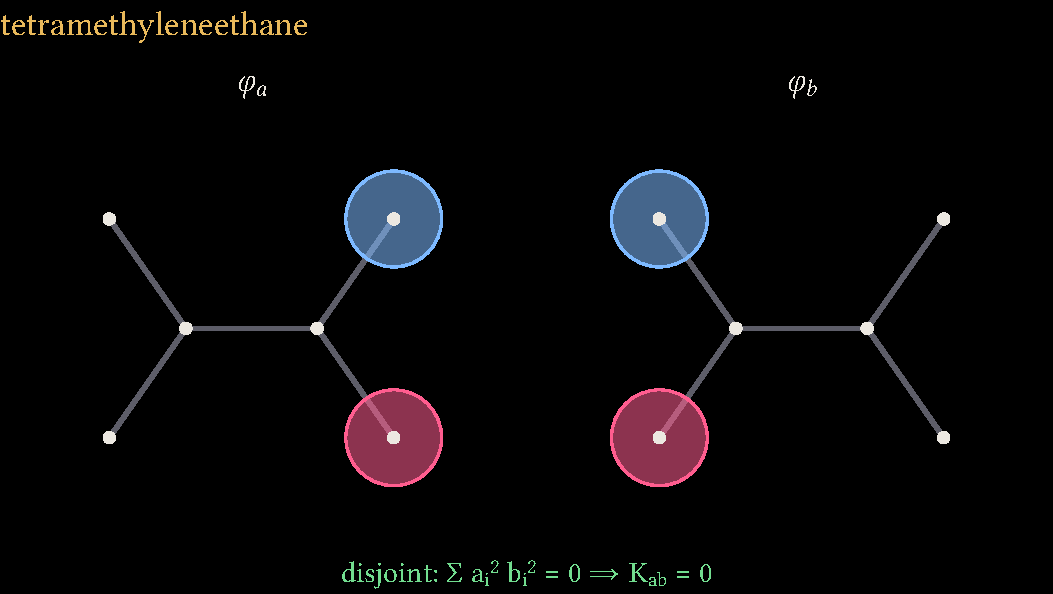
\includegraphics[width=0.53\textwidth]{diagrams/nbmo_tme.pdf}\hfill
  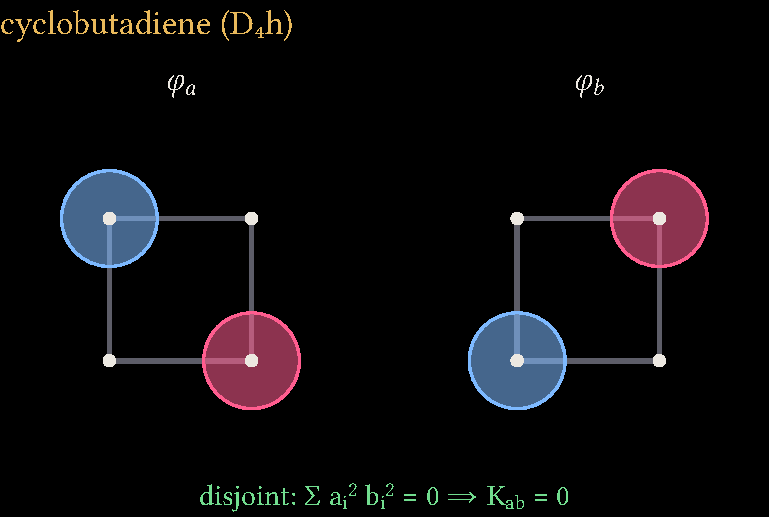
\includegraphics[width=0.44\textwidth]{diagrams/nbmo_cbd.pdf}
  \vskip0.25cm
  \onslide<2->{\small JS code: Hückel matrix $\to$ Jacobi diagonalisation $\to$ rotate the degenerate pair to minimise
    $\sum_ia_i^2b_i^2$ $\to$ SVG $\to$ PDF}
\end{frame}

\begin{frame}{Trimethylenemethane cannot be made disjoint}
  \begin{columns}[c]
    \column{0.5\textwidth}
    \begin{enumerate}
      \item zero-sum at a terminal $\Rightarrow$ $c_0=0$
      \item<2-> zero-sum at the centre $\Rightarrow$ $c_1+c_2+c_3=0$
      \item<3-> a vector in this plane with one nonzero entry cannot sum to zero: \cgold{at least 2 nonzero}
      \item<4-> two such vectors with disjoint supports need $\ge4$ terminal atoms; there are 3
    \end{enumerate}
    \onslide<5->{\centering\crose{nondisjoint, for every choice of basis}\par}
    \column{0.47\textwidth}
    \centering
    \only<5>{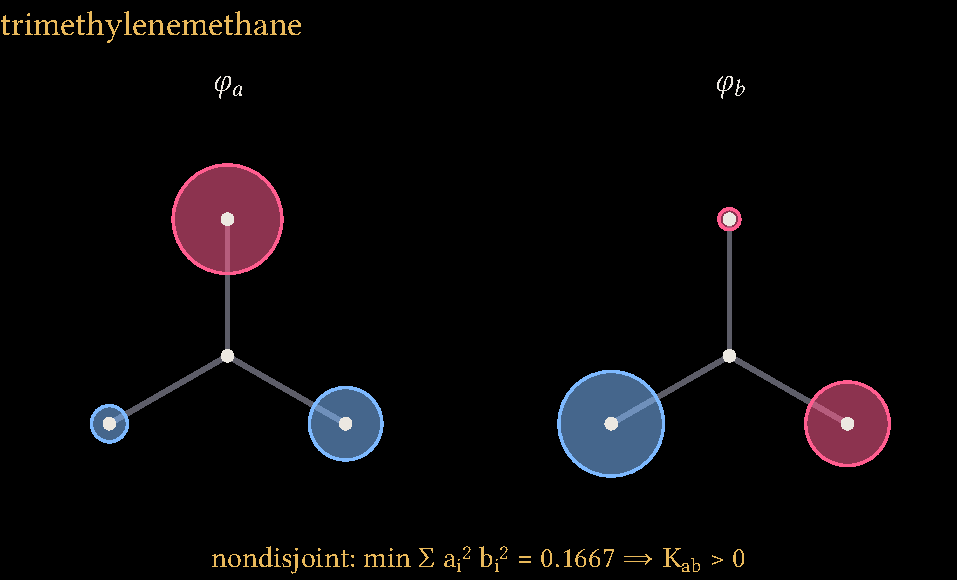
\includegraphics[width=\linewidth]{diagrams/nbmo_tmm.pdf}}
    \only<6->{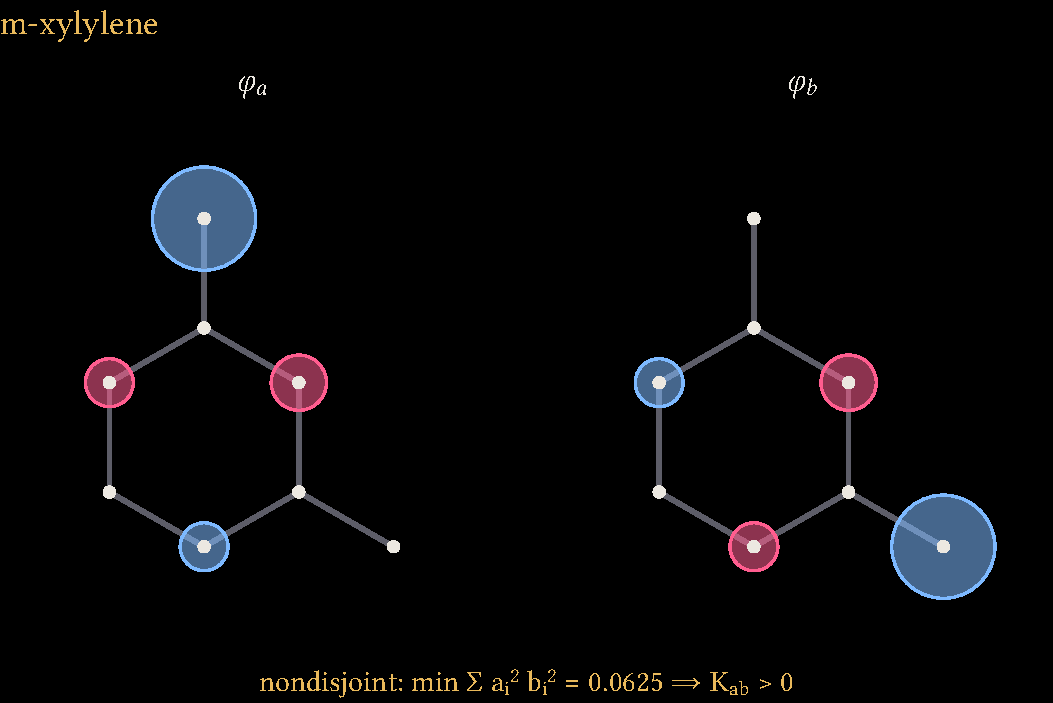
\includegraphics[width=0.9\linewidth]{diagrams/nbmo_mx.pdf}\par
      {\scriptsize\cmuted{$m$-xylylene: also nondisjoint}}}
  \end{columns}
\end{frame}

\begin{frame}{Why disjoint means $K_{ab}=0$}
  \begin{assume}[Zero differential overlap (ZDO)]
    $\eri\mu\nu\lambda\sigma=\delta_{\mu\nu}\delta_{\lambda\sigma}\,\gamma_{\mu\lambda}$, \ $\gamma$ = Coulomb repulsion between atoms $\mu,\lambda$
  \end{assume}
  {\large
  \begin{align*}
    K_{ab}=\eri abab&=\textstyle\sum_{\mu\nu\lambda\sigma}a_\mu b_\nu a_\lambda b_\sigma\,\eri\mu\nu\lambda\sigma\\
    \uncover<2->{}&\uncover<2->{=\textstyle\sum_{\mu\lambda}(a_\mu b_\mu)(a_\lambda b_\lambda)\,\gamma_{\mu\lambda}}\\
    \uncover<3->{\text{disjoint }(a_\mu b_\mu=0\ \forall\mu):\ K_{ab}}&\uncover<3->{=\hlg<3->{0}}\\
    \uncover<4->{\text{Hubbard }(\gamma_{\mu\lambda}=U\delta_{\mu\lambda}):\ K_{ab}}&\uncover<4->{=U\textstyle\sum_\mu a_\mu^2b_\mu^2}
  \end{align*}}
  \onslide<5->{\centering\small TMM: $\min\sum a^2b^2=\tfrac16$ \quad MX: $\tfrac1{16}$ \quad (Python \emph{and} JavaScript agree)\par}
\end{frame}

\begin{frame}{The test: how the gap grows with\ $U$}{T9b: exact Hubbard diagonalisation, $t=1$}
  \begin{columns}[c]
    \column{0.58\textwidth}
    \begin{tikzpicture}
      \begin{loglogaxis}[noirplot,width=7.6cm,height=5.0cm,xmin=0.04,xmax=4.5,
          xlabel={$U/t$},ylabel={$|E_T-E_S|$},ymajorgrids,
          legend style={at={(0.5,-0.3)},anchor=north,legend columns=2}]
        \addplot[noirrose,very thick,mark=*,mark size=1.2pt] table[x=U,y expr=abs(\thisrow{TMM}),col sep=comma]{data/hubbard_gap.csv};
        \addlegendentry{TMM (triplet)}
        \addplot[noirorange,very thick,mark=*,mark size=1.2pt] table[x=U,y expr=abs(\thisrow{MX}),col sep=comma]{data/hubbard_gap.csv};
        \addlegendentry{MX (triplet)}
        \only<2->{\addplot[noircyan,very thick,mark=square*,mark size=1.2pt] table[x=U,y=CBD,col sep=comma]{data/hubbard_gap.csv};}
        \only<2->{\addlegendentry{CBD (singlet)}}
        \only<2->{\addplot[noirgreen,very thick,mark=square*,mark size=1.2pt] table[x=U,y=TME,col sep=comma]{data/hubbard_gap.csv};}
        \only<2->{\addlegendentry{TME (singlet)}}
      \end{loglogaxis}
    \end{tikzpicture}
    \column{0.38\textwidth}
    \begin{itemize}
      \item nondisjoint: slope $\approx1$; \\at $U=0.05$: TMM $0.0164$ vs $2U\cdot\tfrac16=0.0167$
      \item<2-> disjoint: slope $\approx2$ (fit $1.97$, $1.95$), \\singlet below triplet
      \item<3-> first-order $K$ vanishes; something second-order picks the singlet\ldots
    \end{itemize}
  \end{columns}
\end{frame}
